\section{Integral de Superficie}
De nuevo, hemos calculado integrales de funciones cuyo espacio de llegada era $\mathbb{R}$ en conjuntos definidos en $\mathbb{R}^2$. Sin embargo, ¿qué ocurre si el conjunto de integración no es plano sobre $\mathbb{R}^2$ si no que puede ser considerado una superficie en $\mathbb{R}^3$? Además, ¿qué estamos haciendo y cómo si el espacio de llegada es $\mathbb{R}^n$?

\subsection{Concepto de Integral de Superficie}
Para poder responder a las preguntas previas es necesario, de nuevo, acotar el concepto de superficie y ver qué propiedades tiene dicha definición con respecto al concepto de integral.

\begin{defi}[Superficie]
Sea $D \subset  \mathbb{R}^2$ abierto y $\Phi: D \rightarrow \mathbb{R}^3$ una función $C^1$ tal que $\forall \left( u, v \right) \in D : rg\left(D\Phi\left( u, v \right) \right)= 2$, definimos una \textbf{superficie paramétrica} como: 
$$\Phi\left( D \right) = S$$
\end{defi}

\begin{defi}
Diremos que $S$ es una superficie de $A \subset \mathbb{R}^3$ si $A$ es abierto conexo y acotado y $\varphi: A \rightarrow \mathbb{R}^3$ continua.
\begin{itemize}
    \item $\exists B \subset A$ abierto tal que $\varphi$ es $C^1$ sobre $B$.
    \item $\exists K \subset A$ compacto $m\left( K \right) = 0$ tal que $\varphi$ es $C^1$ salvo en un número finito de puntos $L \subset K$.
    \item $S = \varphi\left( B \cup K \right),\ \varphi\left( K \right) \cap \varphi\left( B \right) = \emptyset$.
\end{itemize}
\end{defi}

\begin{obs}
$$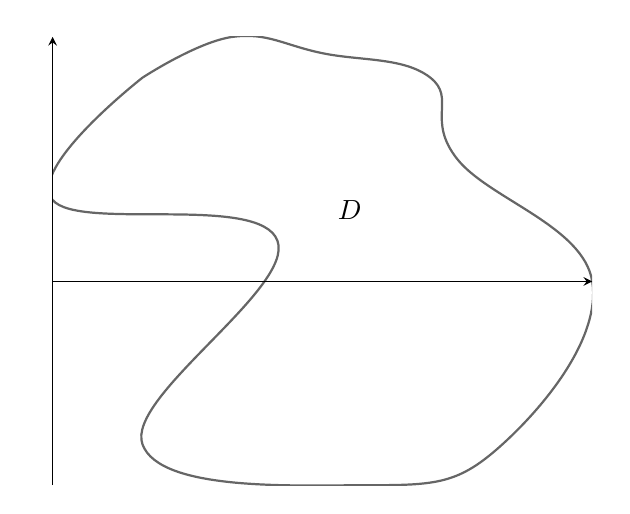
\begin{tikzpicture}
\begin{axis}[
tick style={draw=none},
axis y line=middle,
axis x line=middle,
xticklabels={},yticklabels={}
%grid = both, %major/minor
];
\addplot [thick, domain=-1:8, opacity=0.6]  plot[smooth, tension=.7] coordinates {(2,2.5) (3,3) (4,2.8) (5.2,2.5) (5.5,1.5) (7,0) (6,-2)(4.5,-2.5) (2,-2) (3.5,0.5) (1,1) (2,2.5)};
   

\end{axis}
\node[color=black,right] at (3.5,3.5) {$D$};
\end{tikzpicture}$$
Aplicando $\Phi$  a $D$ obtenemos la superficie paramétrica $S$
$$
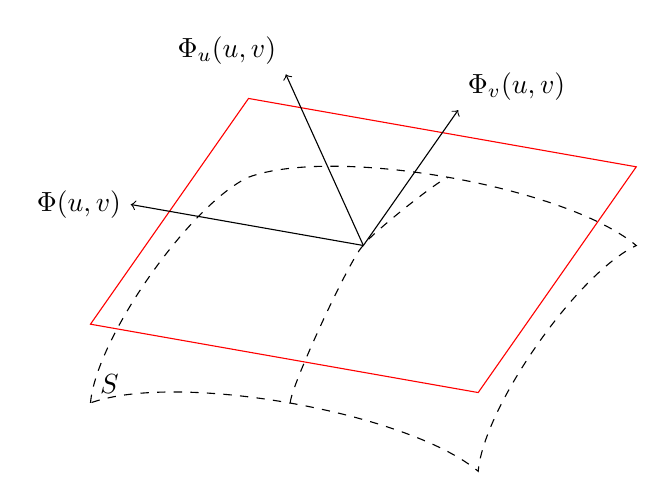
\begin{tikzpicture}[x={(170:1cm)},y={(55:.7cm)},z={(90:1cm)}]
  \draw [red] (2.5,-2.5,0) -- (2.5,2.5,0) -- (-2.5,2.5,0) -- (-2.5,-2.5,0) -- cycle;
  \draw[dashed,looseness=.6] (2.5,-2.5,-1) node[above right] {$S$}
  to[bend left] (2.5,2.5,-1)
  to[bend left] coordinate (mp) (-2.5,2.5,-1)
  to[bend right] (-2.5,-2.5,-1)
  to[bend right] coordinate (mm) (2.5,-2.5,-1)
  -- cycle;
  \draw[dashed,looseness=.2] (mm) to[bend left] (0,0,0) to[bend left] (mp);


  \draw[->] (0,0,0) -- (3,0,0) node[left] {$\Phi (u,v)$};
  \draw[->] (0,0,0) -- (0,3,0) node[above right] {$\Phi_v (u,v)$};
  \draw[->] (0,0,0) -- coordinate[pos=.3] (psi) (1,0,2) node[above left] {$\Phi_u (u,v)$};


\end{tikzpicture}$$
Intuitivamente, estamos diciendo que escogemos un trozo del plano en $\mathbb{R}^2$, lo metemos en $\mathbb{R}^3$ y lo moldeamos como queramos para formar nuestra superficie.

Por la definición que se ha dado, podemos expresar la diferencial como: 
$$\begin{pmatrix} \frac{\partial \Phi_1}{\partial u} & \frac{\partial \Phi_1}{\partial v} \\ \\
\frac{\partial \Phi_2}{\partial u} & \frac{\partial \Phi_2}{\partial v} \\ \\
\frac{\partial \Phi_3}{\partial u} & \frac{\partial \Phi_3}{\partial v} \end{pmatrix} = \begin{pmatrix} \frac{\partial \Phi}{\partial u} & \frac{\partial \Phi}{\partial v} \end{pmatrix} $$
donde las parciales generales sobre $u$ y $v$ son las tangentes sobre la recta en su respectiva coordenada. Precisamente por esto, el espacio generado por $\left\langle \Phi_u, \Phi_v\right\rangle$ es un plano paralelo al tangente a la superficie en ese punto, puesto que los tangentes anteriores son independientes y conforman un sistema generador. El que es realmente será tangente a la superficie es: 
$$\boxed{\Phi \left( u, v \right) + \img D \Phi \left( u, v \right)}$$
Y, por tanto, es razonable pensar que el vector $\frac{\partial\Phi}{\partial u} \times \frac{\partial\Phi}{\partial v}$ será perpendicular a la superficie, por ser perpendicular al plano tangente a la misma.
\end{obs}

\underline{Notación}

A partir de ahora y durante el resto del documento, se utilizarán las siguientes expresiones:
\begin{align*}
\Phi_u = \frac{\partial \Phi}{\partial u} & & \Phi_v = \frac{\partial \Phi}{\partial v}
\end{align*}
para simplificar la complejidad de las expresiones.

\begin{defi}[Área de una superficie]
Dada una superficie $S$ en términos de la caracterización anterior, definimos el \textbf{área} como: 
$$A\left( S \right) = \iint_{D} \lVert \Phi_{u} \times \Phi_v \rVert \dif{u} \dif{v}$$
Cabe destacar que dicha definición coincide\footnote{La demostración se omite por ser muy extensa} con el concepto geométrico de área de una superficie.
\end{defi}

\begin{ej}
Sea $f: \left[ a, b \right] \rightarrow \mathbb{R}$ de $C^1$ y $\forall x \in \left[ a, b \right]: f\left( x \right) \ge 0$, podemos calcular el área generada por su revolución de la siguiente forma:
$$      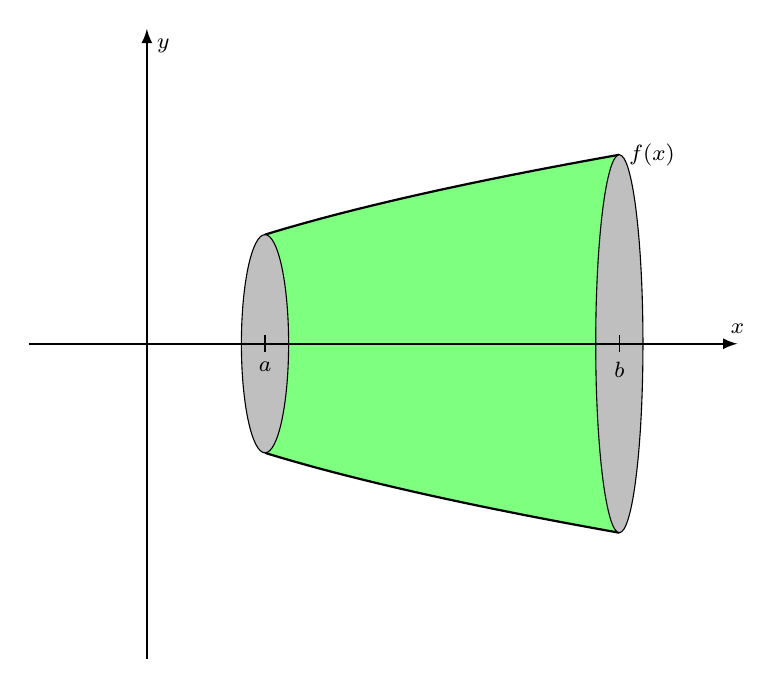
\begin{tikzpicture}[scale=1,>=latex,x=1.5cm,y=0.8cm]
        \fill[fill=green,opacity=0.5] (1,0) -- plot[domain=1:4] (\x,{sqrt(2*(\x)+1))}) -- (4,0);
        \fill[fill=green,opacity=0.5] (1,0) -- plot[domain=1:4] (\x,{-sqrt(2*(\x)+1))}) -- (4,0);
        \draw[-,thick,domain=1:4,samples=100] plot (\x,{sqrt(2*(\x)+1))}) node[right] {\footnotesize $f(x)$};
        \draw[-,thick,domain=1:4,samples=100] plot (\x,{-sqrt(2*(\x)+1))});
        \draw[fill=gray!50] (4,0) circle [x radius =.2 , y radius =3];
        \draw[fill=gray!50] (1,0) circle [x radius =.2 , y radius =1.732050808];

        \draw[->,thick] (-1,0) -- (5,0) node[above] {\footnotesize $x$};
        \draw[->,thick] (0,-5) -- (0,5) node[below right]{\footnotesize $y$};
        \draw[-] (1,3pt) -- (1,-3pt) node[below] {\footnotesize $a$};
        \draw[-] (4,3pt) -- (4,-3pt) node[below] {\footnotesize $b$};
   \draw (0.5,0) node {\AxisRotator}; 
    \end{tikzpicture}$$
En primer lugar, es necesario parametrizar dicha superficie:
$$\Phi: \left( a, b \right) \times \left( 0, 2\pi \right) \rightarrow \mathbb{R}^3$$
$$\Phi \left( u, v \right) = \left( u, f\left( u \right)\cos v, f\left( u \right)\sin v \right) $$
Con esta parametrización, solo renunciamos al borde de puntos de $a$ a $b$ y los puntos del plano horizontal, pero como tienen medida nula no influyen en el resultado, ahora: 
$$\begin{cases}
\Phi_u = \left( 1, f'\left( u \right) \cos v, f'\left( u \right) \sin v \right) \\ \Phi_v = \left( 0, -f\left( u \right) \sin v, f\left( u \right) \cos v \right)
\end{cases}\Rightarrow$$
$$\Phi_u \times \Phi_v = \left( f\left( u \right) f'\left( v \right) \left[ \cos^2 v + \sin^2 v \right], -f\left( u \right) \cos v, -f\left( u \right) \sin v \right)$$
$$\lVert \Phi_u \times \Phi_v \rVert = \sqrt{f\left( u \right)^2 \left[ f'\left( u \right) \right]^2 + f\left( u \right)^2} = f\left( u \right) \sqrt{1 + f'\left( u \right)^2} \Rightarrow$$
$$A\left( S \right) = \int_{a}^{b} \left( \int_{0}^{2\pi} f\left( u \right) \sqrt{1 + f'\left( u \right)^2} \dif{v} \right) \dif{u} = 2\pi \int_{a}^{b} f\left( u \right) \sqrt{1 + f'\left( u \right)^2} \dif{u} $$
Vemos finalmente que la expresión final es, en cierta manera, como integrar las áreas de cada anillo desde $a$ hasta $b$.
\end{ej}

\begin{defi}[Integral sobre una superficie]
Sea $S \subset G \subset \mathbb{R}^3$ donde $G$ es un abierto y $f: G \rightarrow \mathbb{R}$ continua, definimos la \textbf{integral de $f$ sobre $S$} como: 
$$\iint_{S} f \dif{S} = \iint_{D} f\left( \Phi\left( u, v \right) \right) \lVert \Phi_u \times \Phi_v \rVert \dif{u} \dif{v}$$
donde $\Phi: D \rightarrow \mathbb{R}^3$ es la parametrización de $S$.
\end{defi}

\begin{obs}
Si tomamos como $f = 1$, entonces estamos calculando el área de $S$.
\end{obs}

\begin{prop}
Sea $\varphi: G \rightarrow D$ difeomorfismo de $C^1$, entonces: 
$$\Phi \circ \varphi: G \rightarrow S \subset \mathbb{R}^3$$
es una reparametrización.
\end{prop}
\begin{demo}
Tenemos que: 
$$D\left( \Phi \circ \varphi \right) \left( u, v \right) = D\Phi\left( \varphi\left( u, v \right) \right) \circ D\varphi\left( u, v \right)$$
\end{demo}

\begin{prop}
El área de una superficie se mantiene invariante ante reparametrizaciones:
$$\iint_{D} f\left( \left( \Phi \circ \varphi \right) \left( x, y \right) \right) \lVert \left( \Phi \circ \varphi \right)_x \left( \Phi \circ \varphi \right)_y \rVert \dif{x} \dif{y}$$
Este área es la misma puesto que:
$$\lVert \left( \Phi \circ \varphi \right)_x \times \left( \Phi \circ \varphi \right)_y \rVert = \lvert \det D \varphi\left( x, y \right) \rvert \lVert \Phi_u \left( \varphi\left( x, y \right) \right) \times \Phi_v \left( \varphi\left( x, y \right) \right) \rVert$$
\end{prop}

\begin{defi}[Integral de Superficie]
Sea $G \subset \mathbb{R}^3$ un abierto, $S \subset G$ una superficie en él parametrizada por $\Phi: D \rightarrow S$ y $F: G \rightarrow \mathbb{R}^3$ un campo continuo, definimos la \textbf{integral de superficie} de $F$ sobre $S$ a: 
$$\iint_{S} F \dif{\overline{S}} = \iint_{D} F\left( \Phi\left( u, v \right) \right) \cdot \left( \Phi_u \times \Phi_v \right) \dif{u} \dif{v}$$
\end{defi}

\begin{obs}
Del mismo modo que se hizo con las integrales de línea, aquí la idea intuitiva es que $F\left( \Phi\left( u, v \right) \right)$ es el vector que asigna el campo al punto $\Phi\left( u, v \right)$ de la superficie, pues dicho vector se proyecta sobre el vector normal a la superficie en ese punto que es $\Phi_u \times \Phi_v$ y sumamos todos esos vectores. Es decir, si recordamos el producto mixto de vectores, esto es, $a\cdot b\times c$ esta expresión nos daba el volumen del paralelepípedo formado por los 3 vectores, luego de alguna forma estamos sumando los volúmenes generados por un trozo diferencial de superficie.
\begin{center}
    \includegraphics[scale=0.8]{tripleProduct} 
\end{center}Por tanto, esta integral nos permite calcular el \textbf{flujo} del campo que atraviesa la superficie. Además, es necesario tener en cuenta las siguientes características:
\begin{itemize}
    \item El signo de la integral depende de la parametrización, luego habrá que determinar algún sistema para diferenciar la integral.
    \item Si $F$ es tangente a $S \Rightarrow \iint_{S} F \dif{\overline{S}} = 0$.

Para hacer más patente el significado de la integral de superficie vemos que:
$$\iint_{S} F \dif{\overline{S}} = \iint_{D} F\left( \Phi\left( u, v \right) \right) \cdot \left( \Phi_u \times \Phi_v \right) =$$
$$= \iint_{D} F\left( \Phi\left( u, v \right) \right) \cdot \underbrace{\frac{\Phi_u \times \Phi_v}{\lVert \Phi_u \times \Phi_v \rVert}}_{\vec{n}} \cdot \lVert \Phi_u \times \Phi_v \rVert = \iint_{S} F_{\vec{n}} \dif{S}$$
Es decir, estamos haciendo una integral sobre una superficie de la función que proyecta el campo sobre el vector normal.
\end{itemize}
\end{obs}

\begin{prop}
La integral de superficie es invariante por reparametrizaciones siempre que conserven la orientación. De hecho, en caso de que no la conserven únicamente cambia el signo de la integral.
\end{prop}

\begin{ej}
Sea: 
$$\overline{n} = \frac{\Phi_u \times \Phi_v}{\lVert \Phi_u \times \Phi_v \rVert}$$
y también: 
$$S \rightarrow \mathbb{R}^n,\ p \mapsto \begin{cases}
    \vec{n}_p\\
    -\vec{n}_p
\end{cases} $$
Siempre que se pueda hacer esta ``selección'' de forma continua diremos que la superficie es \textbf{orientable}. En el caso de una esfera, solo habrá dos posibles orientaciones.

Como superficie no orientable tenemos la banda de Möbius:
\begin{figure}[H]
\centering    
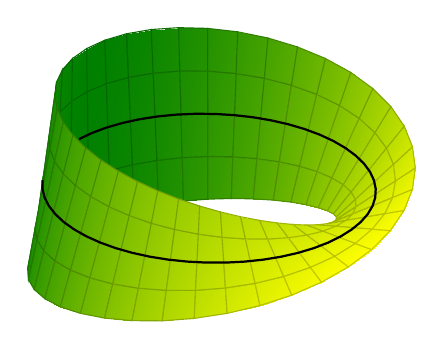
\begin{tikzpicture}
\begin{axis}[
    hide axis,
    view={40}{40}
]
\addplot3 [
    surf, shader=faceted interp,
    point meta=x,
    colormap/greenyellow,
    samples=40,
    samples y=5,
    z buffer=sort,
    domain=0:360,
    y domain=-0.5:0.5
] (
    {(1+0.5*y*cos(x/2)))*cos(x)},
    {(1+0.5*y*cos(x/2)))*sin(x)},
    {0.5*y*sin(x/2)});

\addplot3 [
    samples=50,
    domain=-145:180, % The domain needs to be adjusted manually, depending on the camera angle, unfortunately
    samples y=0,
    thick
] (
    {cos(x)},
    {sin(x)},
    {0});
\end{axis}
\end{tikzpicture}
\caption{\textit{Representación geométrica de una banda de Möbius}}
\end{figure}
\end{ej}

\subsection{Rotacional y Divergencia de un campo}
Se van a desarrollar dos conceptos fundamentales en el análisis vectorial que son la divergencia y el rotacional de un campo. Estos elementos matemáticos son esenciales en áreas como la mecánica de fluidos, la aerodinámica o física y permiten analizar las características que tiene un campo concreto sobre el espacio en el que está definido.

\begin{defi}[Borde de una superficie]
Sea $D$ el recinto interior a una curva $\gamma$ y $\Phi: D \rightarrow \mathbb{R}^3$ la parametrización de una superficie que se puede extender de forma inyectiva y $C^1$ a $\bar{D}$, es decir, a $\partial D$, definimos el \textbf{borde de $S$} como:
$$\partial S = \Phi\left( \partial D \right)$$
Esta definición permite trabajar siempre con conjuntos $D$ muy regulares donde $\partial D$ es una curva cerrada cuyo interior es $D$.
\end{defi}
\begin{obs}
Por la definición que se ha dado, tenemos que: 
$$\left[ a, b \right] \xrightarrow{\gamma} \mathbb{R}^2 \xrightarrow{\Phi} \mathbb{R}^3$$
Luego $\Phi \circ \gamma$ parametriza a la curva $\partial S$, por tanto, es razonable pensar qué orientación inducir a dicha curva para que todo se mantenga uniforme (ya hemos visto que la integral depende de la orientación). Tomemos las siguientes orientaciones: 
    \begin{itemize}
        \item Sabemos la orientación de $S$ a través de $\Phi$. 
        \item Sabemos la orientación de $\gamma$ a través de $D$
    \end{itemize}
Éstas orientaciones determinan una orientación concreta de la curva definida por $\Phi \circ \gamma$. Cuando dada una superficie se toma como orientación de su borde la que viene dada por éste proceso, decimos que la superficie y su borde están orientados de forma compatible.
\end{obs}

\begin{defi}[Rotacional]
Sea el campo $F: \mathbb{R}^3 \rightarrow \mathbb{R}^3$ llamamos \textbf{rotacional} de $F$ a: 
$$\rot F = \nabla \times F = \begin{vmatrix} i & j & k\\
\frac{\partial}{\partial x} & \frac{\partial }{\partial y} & \frac{\partial }{\partial z} \\
F_1 & F_2 & F_3\end{vmatrix} = \left( \frac{\partial F_3}{\partial y} - \frac{\partial F_2}{\partial z}, \frac{\partial F_1}{\partial z} - \frac{\partial F_3}{\partial x}, \frac{\partial F_2}{\partial x} - \frac{\partial F_1}{\partial y} \right)$$
\end{defi}

\begin{obs}
En cierta manera, el rotacional mide la cantidad de giro que provoca el campo en un punto concreto del mismo. Si éste es distinto de 0 hay giro (positivo o negativo determinan el sentido) y si éste es cercano a 0 quiere decir que no hay giro.
\end{obs}

\begin{theo}[de Stokes]
Dada una superficie orientada $S$ con borde orientado de forma compatible y un campo $F$ de clase $C^1$, entonces:
$$\iint_{S} \rot F \dif{\overline{S}} = \int_{\partial S} F \dif{\overline{s}}$$
\end{theo}
\begin{demo}
La demostración se va a hacer para el caso en que la superficie es la gráfica de una función, puesto que es posible demostrar que cualquier superficie se puede poner en términos de otras que sean de esta forma.

Por un lado, la parametrización $\Phi: D \rightarrow \mathbb{R}^3$ de la superficie nos indica que
$$\Phi\left( x, y \right) = \left( x, y, f\left( x, y \right) \right)\Rightarrow \Phi_x \times \Phi_y = \left( \frac{-\partial f}{\partial x}, \frac{-\partial f}{\partial y}, 1\right)$$
la orientación que se toma es hacia las $z$ positivas por ser un 1 la tercera coordenada.

Del mismo modo, tomamos la parametrización $\sigma: I \rightarrow \mathbb{R}^2$ de la curva $\partial D$ de la forma:
$$\sigma\left( t \right) = \left( x\left( t \right), y\left( t \right) \right)$$

Estas dos elecciones, inducen una parametrización en $\partial S$ tal que: 
$$\partial D \xrightarrow{\Phi \circ \sigma} \partial S \stackrel{\Phi \circ \sigma = \gamma}{\Rightarrow} \gamma: I \rightarrow \mathbb{R}^3$$
$$\gamma\left( t \right) = \left( x\left( t \right), y\left( t \right), f\left( x\left( t \right), y\left( t \right) \right) \right)$$

Por tanto, por un lado:
$$\iint_{S} \rot F \dif{\overline{S}} = \int_{D} \rot F \cdot \left( \Phi_x \times \Phi_y \right) \dif{x} \dif{y} =$$
$$= \iint_{D} \left( \left( \frac{\partial F_3}{\partial y} - \frac{\partial F_2}{\partial z} \right) \left( -\frac{\partial f}{\partial x} \right) + \left( \frac{\partial F_1}{\partial z} - \frac{\partial F_3}{\partial x} \right) \left( -\frac{\partial f}{\partial y} \right) + \left( \frac{\partial F_2}{\partial x} - \frac{\partial F_1}{\partial y} \right) \right)$$
Por el otro lado: 
$$\int_{\partial S} F \dif{\overline{s}} = \int_{a}^{b} \left( F_1, F_2, F_3 \right) \cdot \left( x'\left( t \right), y'\left( t \right), \frac{\partial f}{\partial x} x'\left( t \right) + \frac{\partial f}{\partial y} y'\left( t \right) \right) = $$
$$= \int_{a}^{b} \left( F_1x'\left( t \right) - F_2y'\left( t \right) + F_3\left( \frac{\partial f}{\partial x} x'\left( t \right) + \frac{\partial f}{\partial y} y'\left( t \right) \right) \right) \dif{t} = $$
$$= \int_{\partial D} \left( F_1 + F_3 \frac{\partial f}{\partial x} \right) \dif{x} + \left( F_2 + F_3 \frac{\partial f}{\partial y} \right) \dif{y} \stackrel{\text{F. Green}}{=}$$
$$= \iint_{D} \frac{\partial}{\partial x} \left( F_2 + F_3 \frac{\partial f}{\partial y} \right) - \frac{\partial}{\partial y} \left( F_1 + F_3 \frac{\partial f}{\partial x} \right) \dif{x} \dif{y}$$
Y desarrollando se ve que las dos cosas son iguales.
\end{demo}
\begin{obs}
La interpretación geométrica del teorema nos viene de nuevo a remarcar el significado profundo del rotacional: el grado de giro (que viene dado por el rotacional) en un área $S$ es más o menos como:
$$\int_{S} \rot F \dif{\overline{S}} \approx \lVert \rot F \left( p \right) \rVert \cdot Area\left( S \right)$$
pero el teorema dice que se puede calcular también como la integral de línea de $F$ sobre el borde de dicha superficie. Como vimos que la integral de línea era sumar los módulos de las proyecciones del campo sobre las tangentes de la curva, en cierta manera estamos sumando todos los vectores de giro en el borde tal y como muestra el siguiente dibujo:
\begin{center}
    \includegraphics[scale=0.1]{stokeTh} 
\end{center}
\end{obs}

\begin{theo}
Sea $F: \mathbb{R}^3 \rightarrow \mathbb{R}^3 \in C^1$. Son equivalentes: 
\begin{itemize}
    \item $F$ es conservativo.
    \item $\exists f: \mathbb{R}^3 \rightarrow \mathbb{R}$ de $C^2$ de modo que $F = \nabla f$ 
    \item $\rot F = 0$
\end{itemize}
\end{theo}
\begin{demo}
La implicación $1)\Rightarrow 2)$ ya la vimos cuando definimos lo que era un campo conservativo, luego sólo faltan las otras.
\begin{itemize}
\item $2) \Rightarrow 3)$

Esta implicación es inmediata porque el Tª de Schwarz nos asegura que las parciales segundas cruzadas son iguales, luego para $F = \left( \frac{\partial f}{\partial x}, \frac{\partial f}{\partial y}, \frac{\partial f}{\partial z} \right)$, tenemos que:
$$\rot F = \begin{vmatrix} \vec{i} & \vec{j} & \vec{k} \\
\frac{\partial }{\partial x} & \frac{\partial }{\partial y} & \frac{\partial }{\partial z} \\
\frac{\partial f}{\partial x} & \frac{\partial f}{\partial y} & \frac{\partial f}{\partial z} \end{vmatrix} \underbrace{=}_{T. Schwarz} \left( 0, 0, 0 \right)$$

\item $3 \Rightarrow 1)$: 

$$\begin{tikzpicture}
  \begin{axis}[
    axis y line=middle,
axis x line=middle,
%xlabel=$x$,
%grid = both, %major/minor
xticklabels={},yticklabels={},
      xmin=-1.2, xmax=1.2
  ]
  \addplot [middlearrow={latex},domain=-180:180, samples=100, color=blue!50, fill = blue!10, opacity = .5, thick] ({cos(x)},{sin(x)});
  
  \node (n4) at (0.5,0.5) {$S$};
\node (n3) [blue] at (0.9,0.2) {$\partial S = \gamma$};
  \end{axis}
\end{tikzpicture}$$

Sea $S$, si tomamos $\partial S = \gamma$ como curva, entonces por ser el rotacional nulo y el Teorema de Stokes, sabemos que: 
$$\int_{\gamma} F \dif{\overline{s}} = \iint_{S} \rot F \dif{\overline{S}} = 0$$
La demostración no es del todo rigurosa porque falta demostrar que para una curva cualquiera, existe una superficie de la que es borde y esto es más extenso de demostrar (pero cierto).
\end{itemize}
\end{demo}

\begin{obs}
Precisamente de la última observación se deduce que el resultado NO es cierto si $F$ no tiene dominio en todo $\mathbb{R}^3$ o, si se quiere precisar más, si no tiene dominio en un conjunto simplemente conexo (que no haya tubos infinitos que me agujeren una posible superficie).
\end{obs}

\begin{ej}
Sea $G = \mathbb{R}^3 \setminus Z$ y $F: G \rightarrow \mathbb{R}^3$ con $F\left( x, y, z \right) = \left( \frac{-y}{x^2 + y^2}, \frac{x}{x^2 + y^2}, 0 \right)$, vemos que $\rot F = \left( 0, 0, 0 \right)$ porque trivialmente las dos primeras componentes son 0, pero la tercera componente además:
$$\frac{\partial \left( \frac{x}{x^2 + y^2} \right)}{\partial x} - \frac{\partial \left( \frac{-y}{x^2 + y^2} \right)}{\partial y} = \frac{x^2 + y^2 - 2x^2}{\left( x^2 + y^2 \right)^2} + \frac{x^2 + y^2 - 2y^2}{\left( x^2 + y^2 \right)^2} = 0$$
Tomamos la curva:
$$\gamma: \left[ 0, 2\pi \right] \rightarrow \mathbb{R}^3$$
$$\gamma\left( t \right) = \left( \cos t, \sin t, 0 \right)$$
Y vemos que:
$$\int_{\gamma} F \dif{\overline{s}} = \int_{0}^{2\pi} \left( -\sin t, \cos t, 0 \right) \cdot \left( -\sin t, \cos t, 0 \right) \dif{t} = \int_{0}^{2\pi} \cos^2 t + \sin^2t \dif{x} = 2\pi$$
Este ejemplo hace evidente la necesidad de que el dominio sea $\mathbb{R}^3$ ya que no podemos construir una superficie con la curva formada por la circunferencia unidad que no corte al eje Z.
\end{ej} 

%TODO: Ver teorema de la divergencia en R2
\begin{defi}[Divergencia]
Sea $F: G \rightarrow \mathbb{R}^3$ un campo de $C^1$ y $G \subset \mathbb{R}^3$ un abierto, llamamos \textbf{divergencia} de $F$ a: 
$$\divg F = \frac{\partial F_1}{\partial x} + \frac{\partial F_2}{\partial y} + \frac{\partial F_3}{\partial z} = \nabla \cdot F$$
\end{defi}

\begin{obs}
La idea intuitiva detrás del concepto de la divergencia es la cantidad de flujo que sale o entra en un punto del campo, es decir, que para divergencias cercanas a 0 tendremos puntos donde no hay casi flujo de campo, pero para divergencias lejanas a 0 tendremos puntos donde entra más campo o sale más campo (depende del signo).
\end{obs}

\begin{prop}
Sea $H$ un campo $C^2$, entonces $\divg \left( \rot H \right) = 0$. Luego que la divergencia de un campo sea 0 será condición necesaria para ser el rotacional de algún otro.
\end{prop}
\begin{demo}
De nuevo, por el Teorema de Schwarz para las segundas derivadas parciales cruzadas:
$$\divg \left( \underbrace{\frac{\partial H_3}{\partial y} - \frac{\partial H_2}{\partial z}}_{\frac{\partial }{\partial x}}, \underbrace{\frac{\partial H_1}{\partial z} - \frac{\partial H_3}{\partial x}}_{\frac{\partial }{\partial y}}, \underbrace{\frac{\partial H_2}{\partial x} - \frac{\partial H_1}{\partial y}}_{\frac{\partial }{\partial z}} \right) = 0$$
\end{demo}

\begin{theo}
Sea $F: \mathbb{R}^3 \rightarrow \mathbb{R}^3$ un campo de $C^1$ tal que su $\divg F = 0$, entonces $\exists G$ campo de $C^2$ tal que $F = \rot G$.
\end{theo}
\begin{demo}
El $G$ que es rotacional de $F$ viene dado por:
$$\begin{cases}
G_1\left( x, y, z \right) = \displaystyle \int_{0}^{z} F_2\left( x, y, t \right) \dif{t} - \int_{0}^{y} F_3\left( x, t, 0 \right) \dif{t} \\  G_2\left( x, y, z \right) = \displaystyle  -\int_{0}^{z} F_1\left( x, y, t \right) \dif{t} \\ G_3\left( x, y, z \right) = 0
\end{cases}$$
\end{demo}
\begin{obs}
\begin{enumerate}
    \item $G$ no es único, puesto que si tenemos un campo $H$ con $H_3 \neq 0$, entonces $\rot H = F = \rot G \Rightarrow H \neq G$.
    \item El campo gravitatorio es un contraejemplo en el caso de que quitemos un punto del dominio del campo, luego tiene que estar definido en $\mathbb{R}^3$.
\end{enumerate}
\end{obs}

\begin{theo}[de la Divergencia de Gauss]
Sea $\Omega \subset \mathbb{R}^3$ dominio\footnote{Esto quiere decir que $\mathring{\overline{\Omega}} = \mathring{\Omega}$, que $\overline{\Omega} = \overline{\mathring{\Omega}}$ y que $\partial \Omega$ acota a $\Omega$} con la frontera $\partial \Omega$ orientada hacia el exterior y sea $F: G \rightarrow \mathbb{R}^3$ un campo de $C^1$ donde $ \overline{\Omega} \subset G$ y $G$ es un abierto, entonces: 
$$\iint_{\partial \Omega} F \dif{\overline{S}} = \iiint_{\Omega} \divg F$$
\end{theo}
\begin{demo}
Demostremos para el caso en el que suponemos $\Omega = \left\{ \left( x, y, z \right) : f\left( x, y \right) \le z \le g\left( x, y \right) \right\}$ con\\ $f, g : D \rightarrow \mathbb{R}$ de $C^1$, $D \subset \mathbb{R}^2$ y $f \le g$.
$$\begin{tikzpicture}[scale=1]
\def\Anglei{-66}

\draw[thin,->] (-2,0) -- (5,0)  node[above=3pt] {$y$};
\draw[thin,->] (0,-2) -- (0,3)  node[above=3pt] {$z$};

%Zylinder
\begin{scope}[canvas is zx plane at y=0]
\draw[fill=lime,opacity=0.5] (0,2.5) circle (1cm);
\draw[->] (-2,0) -- (3,0)  node[above=3pt] {$x$};
\end{scope}

\begin{scope}[canvas is zx plane at y=1.5]
\path [fill=lime,opacity=0.5] (0,2.5) circle (1cm);
\coordinate (circ1a) at ( $ (0,2.5) + (\Anglei:1cm) $ );
\coordinate (circ1b) at ( $ (0,2.5) + (180+\Anglei:1cm) $ );
\end{scope}

\begin{scope}[canvas is zx plane at y=-1.5]
\path (0,2.5) circle (1cm);
\coordinate (circ2a) at ( $ (0,2.5) + (\Anglei:1cm) $ );
\coordinate (circ2b) at ( $ (0,2.5) + (180+\Anglei:1cm) $ );
\end{scope} 

\begin{scope}[canvas is xy plane at z=0]
\draw (circ1a) -- (circ2a);
\draw (circ1b) -- (circ2b);
\end{scope}

\begin{scope}[canvas is zx plane at y=1.5]
\draw (0,2.5) circle (1cm);
\end{scope}

\begin{scope}[canvas is zx plane at y=-1.5]
\draw (0,2.5) circle (1cm);
\end{scope} 

\begin{scope}[every node/.append style={
xslant=1,sloped}
]
\node at (2.4,-.2) {\scalebox{1}[.7]{Gráfica f}};
\node at (-.8,-.2) {\scalebox{1}[.7]{$\Omega$}};
\node at (3.8, -.2, 3.5) {\scalebox{1}[.7]{D}};
\node at (0.8, -.2, -4.5) {\scalebox{1}[.7]{Gráfica g}};
\end{scope}

\begin{scope}[red]
\node at (3.2, 2.1, 0) {$S_2 \downarrow$};
\node at (3.3, -0.5, 0) {$S_1 \nwarrow$};
\node at (0.9, 0.5, 0) {$S_3 \hookrightarrow$};
\end{scope}

\end{tikzpicture}$$
Sea $F = \left( F_1, F_2, F_3 \right)$ y $\int_{\Omega} \divg F = \int_{\Omega} \left( \frac{\partial F_1}{\partial x} + \frac{\partial F_2}{\partial y} + \frac{\partial F_3}{\partial z} \right) \dif{x} \dif{y} \dif{z}$. En primer lugar, podemos dividir $\partial \Omega = S_1 \cup S_2 \cup S_3$. 
Luego, tenemos que:
$$\int_{\Omega} \frac{\partial F_3}{\partial z} \dif{x} \dif{y} \dif{z} = \int_{D} \left[ \int_{f\left( x, y \right)}^{g\left( x, y \right)} \frac{\partial F_3}{\partial z} \dif{z} \right] \dif{x} \dif{y} = \int_{D} F_3\left( x, y, g\left( x, y \right) \right) - F_3\left( x, y, f\left( x, y \right) \right) \dif{x} \dif{y}$$
Por el otro lado, tenemos:
$$\iint_{\partial \Omega} \left( 0, 0, F_3 \right) \dif{\overline{S}} = \int_{S_1} \left( 0, 0, F_3 \right) + \iint_{S_2} \left( 0, 0, F_3 \right) + \underbrace{\iint_{S_3} \left( 0, 0, F_3 \right)}_{= 0 \text{ (por pendicularidad)}}$$
Parametrizamos la superficie $S_1$, tomando $\Phi: D \rightarrow \mathbb{R}^3$ tal que $\Phi\left( x, y, f\left( x, y \right) \right)$, luego:
$$\begin{cases}
\Phi_x = \left( 1, 0, \frac{\partial f}{\partial x} \right) \\ \Phi_y = \left( 0, 1, \frac{\partial f}{\partial y} \right)
\end{cases}\Rightarrow \Phi_x \times \Phi_y = \left( -\frac{\partial f}{\partial x}, - \frac{\partial f}{\partial y}, 1 \right)$$
Con esto: 
$$\iint_{S_1} \left( 0, 0, F_3 \right) \dif{\overline{S}} = \int_{S_1} \left[ \left( 0, 0, F_3 \right) \cdot n_1 \right] \dif{S} = \iint_{S_1} F_3\left( x, y, f\left( x, y \right) \right) \cdot \frac{- 1}{\sqrt{1 + \left(\frac{\partial f}{\partial x}\right)^2 + \left(\frac{\partial f}{\partial y}\right)^2}} \dif{S} $$
$$= -\iint_{D} F_3\left( x, y, f\left( x, y \right) \right) \frac{1}{\cancel{\sqrt{1 + \frac{\partial f}{\partial x}^2 + \frac{\partial f}{\partial y}^2}}} \cdot \cancel{\sqrt{1 + \frac{\partial f}{\partial x}^2 + \frac{\partial f}{\partial y}^2}} \dif{S} = - \iint_{D} F_3\left( x, y, f\left( x, y \right) \right) \dif{x} \dif{y}$$
Calculando ahora sobre la superficie $S_2$, tenemos que:
$$\iint_{S_2} \left( 0, 0, F_3 \right) \dif{\overline{S}} = \iint_{D} F_3\left( x, y, g\left( x, y \right) \right) \dif{x} \dif{y}$$
Por tanto, hemos probado que:
$$\int_{\Omega} \frac{\partial F_3}{\partial z} \dif{x} \dif{y} \dif{z} = \iint_{\Omega} \left( 0, 0, F_3 \right) \dif{\overline{S}}$$

De modo completamente análogo y escribiéndolo todo para que sean funciones en el otro eje, es decir $(x,z) \mapsto y$, tenemos que: 
$$\begin{tikzpicture}[scale=1]
\def\Anglei{-66}

\draw[thin,->] (-2,0) -- (5,0)  node[above=3pt] {$y$};
\draw[thin,->] (0,-2) -- (0,3)  node[above=3pt] {$z$};

%Zylinder
\begin{scope}[canvas is zx plane at y=0]
\draw[->] (-2,0) -- (3,0)  node[above=3pt] {$x$};
\end{scope}
\begin{scope}
\node[cylinder, draw, shape aspect=.5, 
      cylinder uses custom fill, cylinder end fill=green!50, 
      minimum height=1cm,
      cylinder body fill=green!25, opacity=0.5, 
    scale=1.5, minimum size = 2cm] at (2, 0, 0){};
\end{scope}

\end{tikzpicture}$$


$$\int_{\Omega} \frac{\partial F_2}{\partial y} \dif{x} \dif{y} \dif{z} = \int_{\partial \Omega} \left( 0, F_2, 0 \right) \dif{\overline{S}} $$


Y, de nuevo si consideramos funciones del tipo $(y,z) \mapsto x$

$$\begin{tikzpicture}[scale=1]
\def\Anglei{-66}

\draw[thin,->] (-2,0) -- (5,0)  node[above=3pt] {$y$};
\draw[thin,->] (0,-2) -- (0,3)  node[above=3pt] {$z$};

%Zylinder
\begin{scope}[canvas is zx plane at y=0]
\draw[->] (-5,0) -- (5,0)  node[above=3pt] {$x$};
\end{scope}
\begin{scope}
\node[cylinder, draw, shape aspect=.5, 
      cylinder uses custom fill, cylinder end fill=green!50, 
      minimum height=1cm,
      cylinder body fill=green!25, opacity=0.5, 
    scale=1.5, minimum size = 2cm, rotate = -135] at (0, 0, 0){};
\end{scope}

\end{tikzpicture}$$


$$\int_{\Omega} \frac{\partial F_1}{\partial x} \dif{x} \dif{y} \dif{z} = \int_{\partial \Omega} \left( F_1, 0, 0 \right) \dif{\overline{S}}$$
Consecuentemente, sumando estas últimas ecuaciones obtenemos el resultado del enunciado.
\end{demo}
\begin{obs}
La idea que subyace tras este teorema es que la cantidad de flujo de campo que atraviesa un conjunto $\Omega$ puede expresarse en términos de la divergencia de cada punto de dicho recinto, es decir, como podemos ver aproximado $\iiint_{\Omega} \divg F \dif{x} \dif{y} \dif{z} \approx \divg F\left( p \right) \cdot V\left( \Omega \right)$, entendemos que estamos sumando las divergencias del campo en cada punto de dicho conjunto. El teorema por tanto afirma que calcular eso es lo mismo que calcular el flujo a través de la superficie, que se expresa como $\iint_S F\dif{\overline{S}}$.
\end{obs}
